\documentclass[10pt,twocolumn,letterpaper]{article}
\usepackage[review]{cvpr}
\usepackage{times,graphicx,amsmath,amssymb,booktabs,tabularx,xspace,longtable}
\usepackage[T1]{fontenc}\usepackage{microtype}
\newcolumntype{Y}{>{\raggedright\arraybackslash}X}
\clubpenalty=10000\widowpenalty=10000
\setcounter{topnumber}{5}\setcounter{dbltopnumber}{5}\setcounter{totalnumber}{10}
\renewcommand{\topfraction}{.95}\renewcommand{\dbltopfraction}{.95}\renewcommand{\textfraction}{.05}
\makeatletter\setlength{\@fptop}{0pt}\setlength{\@dblfptop}{0pt}\makeatother
\definecolor{cvprblue}{rgb}{0.13,0.40,0.67}
\usepackage[breaklinks,colorlinks,allcolors=cvprblue]{hyperref}
\def\paperID{Draft}\def\confName{CVPR}\def\confYear{2027}
\title{Brick Atlas: From Static Repair to Autonomous Recovery in Brick Assembly\\Supplementary Material}
\author{Anonymous submission}
\begin{document}\maketitle\raggedbottom
\renewcommand{\thesection}{\Alph{section}}
\renewcommand{\thefigure}{S\arabic{figure}}\renewcommand{\thetable}{S\arabic{table}}
\section{Current Release and Evidence}
This supplement describes the release of 29 October 2026: 310 runnable object configurations, 1,600 static questions, and 3,085 dynamic questions. The collection comprises 263 admitted community configurations and 47 retained designed whole objects. All 4,685 published questions have verified reference executions. These counts supersede earlier manuscript snapshots; they do not convert historical model pilots into results on the current interface.

The release distinguishes three layers: acquired sources, admitted executable configurations, and questions instantiated on them. The source pool has 437 authored objects from 338 original sets, including 99 authored alternatives. Of the 310 runnable configurations, 57 are complete builds and 253 are finishing tasks. A further 174 acquired sources are not admitted to this release. An acquired file is not a runnable benchmark configuration.

The authoritative files are the release manifest, object JSONL, static and dynamic question JSONL, and evaluator-private certificates. The paper snapshots these dependencies in \path{evidence/release-dataset.json}; selected figure states and case IDs are recorded in \path{evidence/release-render-states.json} and \path{evidence/release-figure-selection.json}. Figures are publication exports of exact geometry. Their cameras and lighting do not replace the model's native observations.

\subsection{Historical records and exclusions}
The historical browser preserves 8,997 catalogue records across versions. Only 4,685 are current checked questions; the remainder includes 1,983 retired-source or human-selection records, 2,265 historical records not rechecked, 31 withheld reference/visibility conditions, and 33 pending historical records. This is an archival inventory, not a claim of 8,997 unique valid tasks. Earlier counts such as 5,720 distinct records belong to their own contracts and selected populations.

The 31 withheld designed-object conditions remain in the failure ledger: eighteen do not reach every configured incident under the current reference twelve lack a verified effective change, and one static defect is invisible in all three default views. The current 1,605 retained designed-object questions are the successful subset. One community camper candidate is separately withheld because its original source color cannot be matched without guessing. User-retired buildings and minifigure-containing sources are excluded from admission. No exception is counted as a model failure.

\subsection{Source grouping and overlap}
There are 234 source groups among runnable objects. Authored alternate builds remain in the same group as their original set. Development, validation, and test labels separate source groups, but all current sources have been used during authoring. They therefore do not certify an untouched test distribution. Future external-source evaluation must declare newly acquired source IDs, keep them out of prompt and engine tuning, and report failures in qualification before sampling tasks.

\begin{table*}[t]
\centering\small
\caption{\textbf{Current runnable dataset.} S0/S1 are correct-stage acceptance/static repair; D0/D1/D2 are normal construction/one incident/repeated incidents. Source acquisitions and historical records do not enter these counts.}
\label{tab:dataset}
\begin{tabularx}{\textwidth}{@{}Xrrrrrrr@{}}\toprule
Scope & Objects & S0 & S1 & D0 & D1 & D2 & Questions\\\midrule
Complete build & 57 & 41 & 141 & 57 & 1,466 & 28 & 1,733\\
Finishing task & 253 & 253 & 1,165 & 253 & 1,165 & 116 & 2,952\\
Total & 310 & 294 & 1,306 & 310 & 2,631 & 144 & 4,685\\
\bottomrule
\end{tabularx}
\end{table*}

\begin{table*}[t]
\centering\small
\caption{\textbf{Length descriptors, not calibrated difficulty.} Active parts exclude fixed context.}
\label{tab:length}
\begin{tabularx}{\textwidth}{@{}Xrrr@{}}\toprule
Length & Objects & Static & Dynamic\\\midrule
short (3--7) & 143 & 721 & 884\\
medium (8--15) & 147 & 667 & 1980\\
long (16+) & 20 & 212 & 221\\
\bottomrule
\end{tabularx}
\end{table*}

\begin{table*}[t]
\centering\small
\caption{\textbf{Published question families.} One catalogue family per question; this table is not an exclusive physical-error ontology.}
\label{tab:families}
\begin{tabularx}{\textwidth}{@{}Xrrr@{}}\toprule
Family & Static & Dynamic & Total\\\midrule
buried-repair & 146 & 356 & 502\\
compound & 0 & 122 & 122\\
control & 294 & 310 & 604\\
early-cover & 57 & 57 & 114\\
extra-layer & 80 & 229 & 309\\
left-right-swap & 24 & 24 & 48\\
missing & 262 & 433 & 695\\
multiple & 0 & 144 & 144\\
offset & 156 & 360 & 516\\
repeat-omission & 136 & 136 & 272\\
repeated-step & 78 & 78 & 156\\
rotated & 110 & 225 & 335\\
swapped-positions & 0 & 11 & 11\\
wrong-color & 205 & 389 & 594\\
wrong-part & 52 & 211 & 263\\
\bottomrule
\end{tabularx}
\end{table*}


\section{Construction and Admission Procedure}
\subsection{Representing a complete source}
Community certificates retain source-instance indices, part numbers, colors, and original transforms. Instances are assigned to the operable target, fixed supported context, or conservative background context. The admission check rereads the original file and requires the union of represented indices to equal the complete source instance set. Part aliases are accepted only when resolved part definitions are identical. Raw matrices are checked numerically with a fixed tolerance.

For small complete objects, the target includes every object part and construction begins on a white studded baseplate. For larger sources, the start supplies the body and the scope describes a finishing region. A whole source may contain many more parts than the task operates on. The illustrated gallery retains this body so the remaining work has visible context. Reviewers can choose module focus, whole-object focus, and several angles.

The source pool is audited for minifigure parts. An additional exact structural duplicate check ignores color and translation and normalizes axis-aligned rotations. Its absence of duplicates does not prove that two cars or houses look sufficiently different. Human assessment of meaningful diversity is a separate requirement.

\subsection{Static and dynamic variants}
The community static bank selects a normal stage and distinct faulty states, with two to six questions per admitted object. S0 is a correct intermediate acceptance target, not an invitation to finish all subsequent instructions. S1 uses a supplied faulty state and its stage-specific target. Every question has its own initial and target image paths, so two variants cannot silently display the same stale images.

Dynamic D0 starts normal construction. D1 and D2 retain the same target while specifying one or multiple potential external changes. A reference witness verifies a feasible continuation after each admitted incident. A state-based trigger may defer when an eligible intervention is unavailable. Source diversity and feasible repair determine admission; the generator does not force every error category onto every object.

The family field is a catalogue grouping, not a full causal taxonomy. Missing, color, position, part, and orientation describe discrepancies. Buried repair and early cover describe access demands. Repeated events describe episode structure. Compound errors can involve more than one physical discrepancy. Analyses should preserve these distinctions rather than interpret the table as mutually independent human-error mechanisms.

\subsection{Reference order and reference effort}
The scorer compares physical placement multisets and final constraints. It does not compare the action sequence with a single demonstration. The checker searches adjacent independent swaps in normal reference sequences and verifies successful alternative trajectories for 251 of the 263 community configurations. The remaining twelve may still have other legal orders outside this bounded search.

References support solvability checks and an effort baseline. They are not certified global shortest paths. Removing a correct cover can be necessary; removing an unrelated column can be unnecessary. Human GT review should inspect this distinction. A model taking fewer actions than the recorded reference can be correct and can have a reference-relative effort below one.

\section{Actual Input and Output Contracts}
\subsection{Dynamic initial request}
The Arena initial request contains the task description, starting-state description, sole target contract, neutral physical rules, decision cap, camera metadata, number of inventory and instruction pages, anonymous action handles, and six tool schemas. It does not contain initial RGB automatically. The protocol identifier is \texttt{brick-atlas-tool-arena/3}.

All subsequent replies contain one tool call. The following are syntax examples; identifiers must come from the episode's returned inventory and placement lists. They are separate decisions, not a batch action list.
\begin{quote}\small\ttfamily
\{``tool'':``observe'', ``args'':\{\newline
``view'':``angled'', ``rotateDegrees'':90,\newline
``show'':[``current'',``target'']\}\}\par
\{``tool'':``inspect'', ``args'':\{\newline
``partId'':``A00001'', ``page'':1\}\}\par
\{``tool'':``attach'', ``args'':\{\newline
``partId'':``A00001'',\newline
``candidate'':``C00001''\}\}\par
\{``tool'':``detach'', ``args'':\{\newline
``partId'':``A00001''\}\}\par
\{``tool'':``finish'', ``args'':\{\}\}
\end{quote}
The executable artifact uses standard ASCII JSON quotes. Typeset examples here illustrate the fields; exact copyable requests are in the dataset interface guide and Arena log.

\subsection{Observation semantics}
The angled camera accepts relative rotations of $-90$, $0$, $90$, or $180$ degrees. A top view sets elevation to 90 degrees. Each requested current or target scene is 800 by 600 pixels, with matched camera and scope. The default focus is the operable region; whole focus includes all context. The model can request current, target, and inventory images independently in one observation call.

Inventory contact sheets paginate at twelve parts. Live installed/available status accompanies a requested inventory. Candidate inspection displays possible placements in the actual scene, with the candidate visually outlined. These cards do not label legal or target positions. An instruction-page request returns one optional manual step, marked as a reference rather than the acceptance target. A recall request retrieves previously requested images and their original decision number; it does not observe the current state.

After attach or detach, feedback describes acceptance, physical rejection, resource rejection, or invalid parameters. No fresh scene image is attached automatically. The model can continue building without looking or spend a decision to observe. The spectator page's three-angle images are generated for review and are not implicitly delivered to the model.

\subsection{Static adapter}
Static tasks initially provide three matched current/target views and an inventory contact sheet. Responses use \texttt{type}, rather than the dynamic envelope's \texttt{tool} and \texttt{args}. For example, \texttt{\{``type'':``finish''\}} submits acceptance; inspect, attach, and detach expose the same underlying scene semantics. The different sensing policies are versioned. Claims that static and dynamic scores isolate only an intervention require an additional matched-sensor experiment.

\subsection{Public and evaluator-private data}
The public model request may reveal anonymous inventory and placement handles, optional instructions, requested RGB, and neutral action feedback. It must not reveal error-family labels, hidden schedules, reference actions, private goal dictionaries, event counts, or evaluator success signals while the episode is active. Human review pages can show GT separately; they are explicitly answer-bearing surfaces. Trace exports record what the model actually saw rather than substituting spectator images.

\section{Metrics and Denominators}
\subsection{Exact completion and partial state quality}
Placement signatures contain part type, color, and world pose, with multiplicities for interchangeable parts. Fixed context is not included in operable-placement F1. Exact success requires explicit finish, equality with the target signature, and any final connection constraints. An accepted off-target move is legal but may need later correction; it is not an automatic failure.

For static S1, report exact SR, full-placement F1, initial and final residual, error reduction, originally missing target content recovered, original excess cleared, and final damage to initially correct placements. Residual is the number of missing and excess placements. It is not shortest repair distance. Error reduction is undefined for an initially exact state and can be negative after deterioration. S0 separately reports correct acceptance and whether any physical move was accepted.

\subsection{Dynamic normal and incident runs}
BCR uses valid D0 runs. ICR is valid completion of incident-assigned runs, irrespective of whether the incident was reached. Trigger coverage retains scheduled and applied counts. The primary normal-qualified recovery measure further requires a successful matched normal run, a valid terminal status, complete incident exposure, and verified effective change. Its success field remains null when ineligible.

The matched normal and incident runs share the task, evaluated model, input contract, and budget, but are independently executed. This supports a descriptive conditional recovery rate. It does not support a causal completion drop. A strict paired estimator requires real evidence of a cloned prefix, including messages and already spent budget. The scorer supports that distinction; a completed shared-prefix agent study is not supplied by this release.

\subsection{Event windows}
An event window starts after the incident and ends immediately before the next incident. Lost correct content is measured relative to the before-event state and the final target; introduced excess is measured relative to pre-existing excess. Recovery can coexist with forward progress. It need not reproduce the old prefix exactly.

First recovery is counted in subsequent decisions, including observations and invalid actions. Retention requires at least two follow-up decisions. Observed relapse fails retention; insufficient follow-up yields N/A. Pure access obstructions without a new placement defect use completion-related evaluation instead of declaring instantaneous recovery. For repeated incidents, partial exposure and incomplete later recovery remain explicit.

\subsection{Failures and aggregation}
The terminal statuses eligible for ability evaluation are completed and model-budget-exhausted. A wrong explicit finish or exhausted model budget is failure. Service error, harness error, and external stop are separate technical outcomes. Format errors and schema errors are distinct from collisions, inaccessible paths, wrong placements, and out-of-stock responses. Recovery cannot be used as a direct detection label.

Every model table should provide planned attempts, valid attempts, event exposure, and metric eligibility. Report task-micro and object/source-macro results. Source-clustered intervals preserve correlated variants. A single run per condition describes that run and the sampled task set; it does not quantify within-model run variance. Cost totals include observation images, instruction pages, recalls, retries, prompt/history tokens, generated tokens, and local computation when applicable.

\section{Verification and Remaining Checks}
Reference replay verifies all published questions and source consistency. The image audit verifies 17,618 scene assets and current/target agreement in size. Normal controls match exactly. Community static defects differ in at least one exported view. This nonempty-pixel test does not establish human salience, nor does a finite set of views prove that every adaptive event is visible at every runtime location.

Six actual ToolArena scripted episodes cover three objects with normal and incident conditions: the complete cow, a truck finishing task, and a longer building task. They exercise real tool envelopes, requested images, action feedback, terminal scoring, and normal-qualified recovery. These are privileged witnesses; they use reference knowledge and are never reported as learned-agent successes. The final check also runs metric and contract regressions for alternative orders, correct intermediate acceptance, untriggered events, incomplete exposure, and technical failures.

Independent human checks must distinguish displayed-GT review from blind operation. Reviewers first assess whether the target and operable region are clear, then whether the proposed repair changes the right parts without unnecessary collateral work. Blind operators receive only model-visible evidence and controls. Their outcomes establish usability and ability, while GT agreement only supports annotation quality. No copied agreement from one reviewer supplies another independent observation.

Independent mechanical checking should examine buried parts, interlocking geometry, conservative background collisions, extraction paths, and whether removing a support invalidates other parts. The present engine uses fixtures and does not simulate gravitational collapse or deformation. No program-only audit is labeled independent physical validation.

\section{Planned Experiments and Empty Result Sheets}
Nineteen result sheets remain unmeasured; dashes are not zeros. Machine-readable fields in \path{evidence/release-results-template.json} are null. The ten inherited candidate labels are shown below. Pin exact model versions, access, preprocessing, decoding, and budgets before one run per condition. No new API calls were made. Planned checkpoint, text-state, coordinate, detection, cross-agent, and shared-prefix studies require integration; their tables state these limits.

\clearpage
\begin{table*}[!ht]
\centering\small
\caption{\textbf{E1: static repair (unmeasured).} Implemented. Separate whole-object and finishing stages; SR/F1/ER/DR use S1 and FR uses S0. Dashes mean not run, never zero.}
\begin{tabularx}{\textwidth}{@{}Xrrrrrr@{}}\toprule
Model & SR & F1 & ER & DR & S0 FR & Valid N\\\midrule
GPT-6.1 Sol & --- & --- & --- & --- & --- & ---\\
Claude Sonnet 5.5 & --- & --- & --- & --- & --- & ---\\
Gemini 3.8 Flash & --- & --- & --- & --- & --- & ---\\
Claude Haiku 5.5 & --- & --- & --- & --- & --- & ---\\
Qwen3.5-9B & --- & --- & --- & --- & --- & ---\\
Qwen3.5-27B & --- & --- & --- & --- & --- & ---\\
InternVL3.5-8B & --- & --- & --- & --- & --- & ---\\
Qwen2.5-VL-7B & --- & --- & --- & --- & --- & ---\\
Qwen2.5-VL-32B & --- & --- & --- & --- & --- & ---\\
Gemma 3-12B & --- & --- & --- & --- & --- & ---\\
\bottomrule
\end{tabularx}
\end{table*}
\begin{table*}[t]
\centering\small
\caption{\textbf{E2: dynamic construction and recovery (unmeasured).}  W/M: whole-object/named-module scope. BCR uses D0; CRR requires normal success and verified complete exposure; $\Delta$ uses eligible pairs without filtering control success. Report D1 and D2 separately. ICR, TR and eligibility counts are retained in E3/E6/E9 and the ledger.}
\label{tab:dynamic-main}
\begin{tabularx}{\textwidth}{@{}Xrrrrrr@{}}
\toprule
Model & W BCR & W CRR & W $\Delta$ & M BCR & M CRR & M $\Delta$\\
\midrule
GPT-6.1 Sol & --- & --- & --- & --- & --- & ---\\
Claude Sonnet 5.5 & --- & --- & --- & --- & --- & ---\\
Gemini 3.8 Flash & --- & --- & --- & --- & --- & ---\\
Claude Haiku 5.5 & --- & --- & --- & --- & --- & ---\\
Qwen3.5-9B & --- & --- & --- & --- & --- & ---\\
Qwen3.5-27B & --- & --- & --- & --- & --- & ---\\
InternVL3.5-8B & --- & --- & --- & --- & --- & ---\\
Qwen2.5-VL-7B & --- & --- & --- & --- & --- & ---\\
Qwen2.5-VL-32B & --- & --- & --- & --- & --- & ---\\
Gemma 3-12B & --- & --- & --- & --- & --- & ---\\
\bottomrule
\end{tabularx}
\end{table*}
\begin{table}[t]
\centering\small
\caption{\textbf{E2: paired intervention effect (unmeasured).} Same-prefix control/fault branches. $n$: exposed pairs; $\Delta=C_c-C_f$: signed completion drop in percentage points. Expand to all ten models; these three are selected before evaluation.}
\label{tab:paired}
\begin{tabularx}{\linewidth}{@{}Xrrrr@{}}
\toprule
Model & D $n$ & D $\Delta$ & M $n$ & M $\Delta$\\
\midrule
Sol & --- & --- & --- & ---\\
Flash & --- & --- & --- & ---\\
Qwen 27B & --- & --- & --- & ---\\
\bottomrule
\end{tabularx}
\end{table}

\clearpage
\begin{table}[t]
\centering\small
\caption{\textbf{E3: input ablations (unmeasured).} Each cell reports D/M recovery; use identical cases and seeds. Sol = GPT-6.1 Sol; Argon = Gemini 4 Argon; Qwen = Qwen3.5-27B. M-only manual ablation has no D value. Symbolic input is privileged.}
\label{tab:ablations}
\begin{tabularx}{\linewidth}{@{}Xrrr@{}}
\toprule
Input condition & Sol & Argon & Qwen\\
\midrule
Full visual interface & --- & --- & ---\\
No previous image & --- & --- & ---\\
No manual (M only) & n/a / --- & n/a / --- & n/a / ---\\
No candidate preview & --- & --- & ---\\
Success/failure feedback & --- & --- & ---\\
Symbolic state & --- & --- & ---\\
\bottomrule
\end{tabularx}
\end{table}
\begin{table*}[t]
\centering\small
\caption{\textbf{E9: static error breakdown (unmeasured).} Counts are definitions in the current 467-question S test split, not the 3,292-question bank. Instantiate per named model, with one run per case and source-macro completion. Sparse categories are descriptive; repair-state replacements are reported separately.}
\label{tab:staticerrors}
\begin{tabularx}{\textwidth}{@{}Xrrrr@{}}
\toprule
S category & Definitions & Completed / trials & Success & 95\% CI\\
\midrule
Compound & 147 & --- & --- & ---\\
Normal control & 23 & --- & --- & ---\\
Extra piece & 2 & --- & --- & ---\\
Layer height & 13 & --- & --- & ---\\
Missing & 95 & --- & --- & ---\\
Offset & 38 & --- & --- & ---\\
Replacement repair state & 17 & --- & --- & ---\\
Rotation & 35 & --- & --- & ---\\
Swapped positions & 3 & --- & --- & ---\\
Wrong color & 71 & --- & --- & ---\\
Wrong size & 6 & --- & --- & ---\\
Wrong type & 17 & --- & --- & ---\\
\bottomrule
\end{tabularx}
\end{table*}
\begin{table*}[t]
\centering\small
\caption{\textbf{E6: dynamic errors (unmeasured).}  W/M assignment counts are multilabel. The module-swap cell has zero assigned tasks and yields N/A, not a model failure. ICR uses valid assigned runs; CRR and $\Delta$ use their declared paired populations.}
\label{tab:dynamic-errors}
\begin{tabularx}{\textwidth}{@{}Xrrrrrr@{}}
\toprule
Label & W assigned & M assigned & ICR & TR & CRR & $\Delta$\\
\midrule
E01 Missing & 209 & 60 & --- & --- & --- & ---\\
E02 Extra & 167 & 36 & --- & --- & --- & ---\\
E03 Color & 426 & 60 & --- & --- & --- & ---\\
E04 Part & 185 & 15 & --- & --- & --- & ---\\
E05 Position & 227 & 32 & --- & --- & --- & ---\\
E06 Orientation & 130 & 25 & --- & --- & --- & ---\\
E07 Swap & 20 & 0 & --- & --- & --- & ---\\
\bottomrule
\end{tabularx}
\end{table*}

\clearpage
\begin{table*}[t]
\centering\small
\caption{\textbf{E10: correction quality and collateral damage (unmeasured).} For S and M-static, report terminal defect reduction (DR), target-multiset part F1, exact completion, new damage to initially correct placements (CD), and unnecessary edits on normal controls (UE). Report S and M-static separately; dynamic recovery is reported separately in E1/E2. Temporary removals are allowed; CD measures terminal damage only.}
\label{tab:repairquality}
\begin{tabularx}{\textwidth}{@{}Xrrrrr@{}}
\toprule
Model & DR $\uparrow$ & Part F1 $\uparrow$ & Exact $\uparrow$ & CD $\downarrow$ & UE $\downarrow$\\
\midrule
GPT-6 Astra & --- & --- & --- & --- & ---\\
GPT-6.1 Sol & --- & --- & --- & --- & ---\\
GPT-6 Luna & --- & --- & --- & --- & ---\\
Claude Opus 5.5 & --- & --- & --- & --- & ---\\
Claude Sonnet 5.5 & --- & --- & --- & --- & ---\\
Claude Haiku 5.5 & --- & --- & --- & --- & ---\\
Gemini 4 Argon & --- & --- & --- & --- & ---\\
Gemini 3.8 Flash & --- & --- & --- & --- & ---\\
Qwen3.5-9B & --- & --- & --- & --- & ---\\
Qwen3.5-27B & --- & --- & --- & --- & ---\\
InternVL3.5-8B & --- & --- & --- & --- & ---\\
InternVL3.5-38B & --- & --- & --- & --- & ---\\
\bottomrule
\end{tabularx}
\end{table*}
\begin{table}[t]
\centering\small
\caption{\textbf{E8: structural strata (unmeasured).}  Counts include all main candidates. Static B uses the stage target; R uses a feasible witness. Report outcomes by track/task type rather than pooling these strata into one score. G is provisional, not measured difficulty.}
\label{tab:difficulty}
\begin{tabularx}{\linewidth}{@{}Xrrrr@{}}
\toprule
Stratum & Assigned & SR/BCR & CRR & Eligible $N$\\
\midrule
B1 & 4873 & --- & --- & ---\\
B2 & 531 & --- & --- & ---\\
B3 & 48 & --- & --- & ---\\
R0 & 323 & --- & --- & ---\\
R1 & 2656 & --- & --- & ---\\
R2 & 411 & --- & --- & ---\\
R3 & 2062 & --- & --- & ---\\
T0 & 3760 & --- & --- & ---\\
T1 & 1649 & --- & --- & ---\\
T2 & 37 & --- & --- & ---\\
T3 & 6 & --- & --- & ---\\
G1 & 2577 & --- & --- & ---\\
G2 & 2823 & --- & --- & ---\\
G3 & 52 & --- & --- & ---\\
\bottomrule
\end{tabularx}
\end{table}
\begin{table*}[t]
\centering\small
\caption{\textbf{E9: repeated incidents (unmeasured).} Implemented event windows end before the next external incident; short retention windows are N/A. Dashes mean not run, never zero.}
\begin{tabularx}{\textwidth}{@{}Xrrrrr@{}}\toprule
Model & All-event SR & Exposure & Recovered & Retention & Eligible N\\\midrule
GPT-6.1 Sol & --- & --- & --- & --- & ---\\
Claude Sonnet 5.5 & --- & --- & --- & --- & ---\\
Gemini 3.8 Flash & --- & --- & --- & --- & ---\\
Claude Haiku 5.5 & --- & --- & --- & --- & ---\\
Qwen3.5-9B & --- & --- & --- & --- & ---\\
Qwen3.5-27B & --- & --- & --- & --- & ---\\
InternVL3.5-8B & --- & --- & --- & --- & ---\\
Qwen2.5-VL-7B & --- & --- & --- & --- & ---\\
Qwen2.5-VL-32B & --- & --- & --- & --- & ---\\
Gemma 3-12B & --- & --- & --- & --- & ---\\
\bottomrule
\end{tabularx}
\end{table*}

\clearpage
\begin{table*}[t]
\centering\small
\caption{\textbf{E10: checkpoint continuation (planned bank).}  The system builds the prefix; this is not agent-built progress. No independent C bank or current CSR results exist. Repair@k requires adequate observation windows; censoring is separate.}
\label{tab:checkpoint}
\begin{tabularx}{\textwidth}{@{}Xrrrrr@{}}
\toprule
Scope & CSR & Repair@2 & @4 & @8 & Valid $N$\\
\midrule
Whole object & --- & --- & --- & --- & ---\\
Named module & --- & --- & --- & --- & ---\\
\bottomrule
\end{tabularx}
\end{table*}
\begin{table*}[!ht]
\centering\small
\caption{\textbf{E11: static input representation (unmeasured).} Planned adapters. First three compare native interfaces with unequal perceptual information; last three encode identical facts and test representation/OCR. Keep family and visibility strata; never pool the two studies. Dashes mean not run, never zero.}
\begin{tabularx}{\textwidth}{@{}Xrrrrr@{}}\toprule
Input & S1 SR & F1 & S0 FR & Damage & Valid N\\\midrule
T: structured text & --- & --- & --- & --- & ---\\
I: native scene images & --- & --- & --- & --- & ---\\
TI: both & --- & --- & --- & --- & ---\\
T: matched fact ledger & --- & --- & --- & --- & ---\\
I: rendered fact cards & --- & --- & --- & --- & ---\\
TI: matched facts in both & --- & --- & --- & --- & ---\\
\bottomrule
\end{tabularx}
\end{table*}
\begin{table*}[t]
\centering\small
\caption{\textbf{E12: output localization (planned).}  Coordinates add pose estimation to action choice. Build the coordinate adapter and matched cases before comparison. Keep geometry, goals, and information fixed.}
\label{tab:action-output}
\begin{tabularx}{\textwidth}{@{}Xrrrr@{}}
\toprule
Output & SR/BCR & CRR & Schema errors & Valid $N$\\
\midrule
Anonymous candidate ID & --- & --- & --- & ---\\
Free position + orientation & --- & --- & --- & ---\\
\bottomrule
\end{tabularx}
\end{table*}

\clearpage
\begin{table*}[t]
\centering\small
\caption{\textbf{E11: separate detection/localization probe (unmeasured).} Fixed certified snapshots from the 24 D/M control/fault pairs give 48 conditions. Queries never interrupt assembly. BA: balanced change-detection accuracy; TPR/FPR: anomaly recall/false alarms; Loc: affected piece/slot F1. Independent human readability is recorded with the same images.}
\label{tab:perceptionprobe}
\begin{tabularx}{\textwidth}{@{}Xrrrrr@{}}
\toprule
Agent & BA & TPR & FPR & Loc & Readable\\
\midrule
Independent humans & --- & --- & --- & --- & ---\\
GPT-6 Astra & --- & --- & --- & --- & ---\\
GPT-6.1 Sol & --- & --- & --- & --- & ---\\
GPT-6 Luna & --- & --- & --- & --- & ---\\
Claude Opus 5.5 & --- & --- & --- & --- & ---\\
Claude Sonnet 5.5 & --- & --- & --- & --- & ---\\
Claude Haiku 5.5 & --- & --- & --- & --- & ---\\
Gemini 4 Argon & --- & --- & --- & --- & ---\\
Gemini 3.8 Flash & --- & --- & --- & --- & ---\\
Qwen3.5-9B & --- & --- & --- & --- & ---\\
Qwen3.5-27B & --- & --- & --- & --- & ---\\
InternVL3.5-8B & --- & --- & --- & --- & ---\\
InternVL3.5-38B & --- & --- & --- & --- & ---\\
\bottomrule
\end{tabularx}
\end{table*}
\begin{table*}[t]
\centering\small
\caption{\textbf{E14: repair of another agent state (unmeasured).} Planned shared failed-state bank with matched checkpoints and no hidden reference access. Dashes mean not run, never zero.}
\begin{tabularx}{\textwidth}{@{}Xrrrr@{}}\toprule
Repairer & Own state SR & Other state SR & Residual & Valid N\\\midrule
GPT-6.1 Sol & --- & --- & --- & ---\\
Claude Sonnet 5.5 & --- & --- & --- & ---\\
Gemini 3.8 Flash & --- & --- & --- & ---\\
Claude Haiku 5.5 & --- & --- & --- & ---\\
Qwen3.5-9B & --- & --- & --- & ---\\
Qwen3.5-27B & --- & --- & --- & ---\\
InternVL3.5-8B & --- & --- & --- & ---\\
Qwen2.5-VL-7B & --- & --- & --- & ---\\
Qwen2.5-VL-32B & --- & --- & --- & ---\\
Gemma 3-12B & --- & --- & --- & ---\\
\bottomrule
\end{tabularx}
\end{table*}
\begin{table}[t]
\centering\small
\caption{\textbf{E15: observation robustness (unmeasured).}  Keep camera/geometry fixed for resolution tests; restrict inspection too for single-view tests. Record delivered images and recheck visibility. Repeat separately by track and task type.}
\label{tab:visual}
\begin{tabularx}{\linewidth}{@{}Xrrr@{}}
\toprule
Condition & SR/BCR & CRR & Valid $N$\\
\midrule
Native comparison canvas & --- & --- & ---\\
One fixed view & --- & --- & ---\\
No previous scene & --- & --- & ---\\
Half image resolution & --- & --- & ---\\
Double image resolution & --- & --- & ---\\
\bottomrule
\end{tabularx}
\end{table}

\clearpage
\begin{table*}[t]
\centering\small
\caption{\textbf{E16: planning and budget (unmeasured).} Planned study; charge all decisions and queries, and change one budget at a time. Dashes mean not run, never zero.}
\begin{tabularx}{\textwidth}{@{}Xrrrrr@{}}\toprule
Condition & SR & BCR & NQR & Decisions & USD\\\midrule
Default decision cap & --- & --- & --- & --- & ---\\
Half decision cap & --- & --- & --- & --- & ---\\
Double decision cap & --- & --- & --- & --- & ---\\
Observation schedule & --- & --- & --- & --- & ---\\
\bottomrule
\end{tabularx}
\end{table*}
\begin{table*}[t]
\centering\small
\caption{\textbf{E17: cost and action efficiency (unmeasured).}  Include shared prefixes, both continuations, billed errors and retries. Attempt/reference is relative to a feasible witness, not proven optimality. Repeat per scope, task type, and model.}
\label{tab:efficiency}
\begin{tabularx}{\textwidth}{@{}Xrrrrrr@{}}
\toprule
Model & Decisions & Inspect & Attempt/ref. & Image tokens & USD/task & USD/success\\
\midrule
GPT-6.1 Sol & --- & --- & --- & --- & --- & ---\\
Claude Sonnet 5.5 & --- & --- & --- & --- & --- & ---\\
Gemini 3.8 Flash & --- & --- & --- & --- & --- & ---\\
Claude Haiku 5.5 & --- & --- & --- & --- & --- & ---\\
Qwen3.5-9B & --- & --- & --- & --- & --- & ---\\
Qwen3.5-27B & --- & --- & --- & --- & --- & ---\\
InternVL3.5-8B & --- & --- & --- & --- & --- & ---\\
Qwen2.5-VL-7B & --- & --- & --- & --- & --- & ---\\
Qwen2.5-VL-32B & --- & --- & --- & --- & --- & ---\\
Gemma 3-12B & --- & --- & --- & --- & --- & ---\\
\bottomrule
\end{tabularx}
\end{table*}
\begin{table}[t]
\centering\small
\caption{\textbf{E18: independent human operation (planned).}  Graphical actions only. The proposed 72-condition panel spans static, whole-dynamic, and module-dynamic tasks; six participants provide three observations per condition without seeing both pair members. Current task selection and schedules require qualification.}
\label{tab:human}
\begin{tabularx}{\linewidth}{@{}Xrrrr@{}}
\toprule
Agent & Static SR & BCR & CRR & Valid $N$\\
\midrule
Human (independent) & --- & --- & --- & ---\\
Sol & --- & --- & --- & ---\\
Flash & --- & --- & --- & ---\\
Qwen 27B & --- & --- & --- & ---\\
\bottomrule
\end{tabularx}
\end{table}
\begin{table}[t]
\centering\small
\caption{\textbf{E19: validity and failure ledger (unmeasured).}  Format, schema/IDs, physics, construction, exposure, and service outcomes are separate. Categories can co-occur; do not force their sum to equal failure N.}
\label{tab:failures}
\begin{tabularx}{\linewidth}{@{}Xrr@{}}
\toprule
Record & Count & Rate / coverage\\
\midrule
Planned / valid attempts & --- & ---\\
Parsing errors & --- & ---\\
Schema / handle errors & --- & ---\\
Physical rejections & --- & ---\\
Normal controls failed & --- & ---\\
Events untriggered & --- & ---\\
Events partially triggered & --- & ---\\
Incident effect unverified & --- & ---\\
Eligible CRR pairs & --- & ---\\
Model budget exhausted & --- & ---\\
Final service error & --- & ---\\
Harness error / external stop & --- & ---\\
\bottomrule
\end{tabularx}
\end{table}

\clearpage
\onecolumn
\section{Complete Runnable Object Inventory}
The gallery below contains every runnable configuration, followed by its stable ID, scope, active-part count, and question counts. Native release overview images retain the source context; the interactive review page additionally exposes focused current/target pairs, three angles, question-specific GT, and deep links. A tiny thumbnail is an inventory aid, not the image used for judging a defect. All 310 IDs are present in the current object index. Source attribution, original titles, and licenses remain in the machine-readable catalogue.
\begin{figure}[!ht]\centering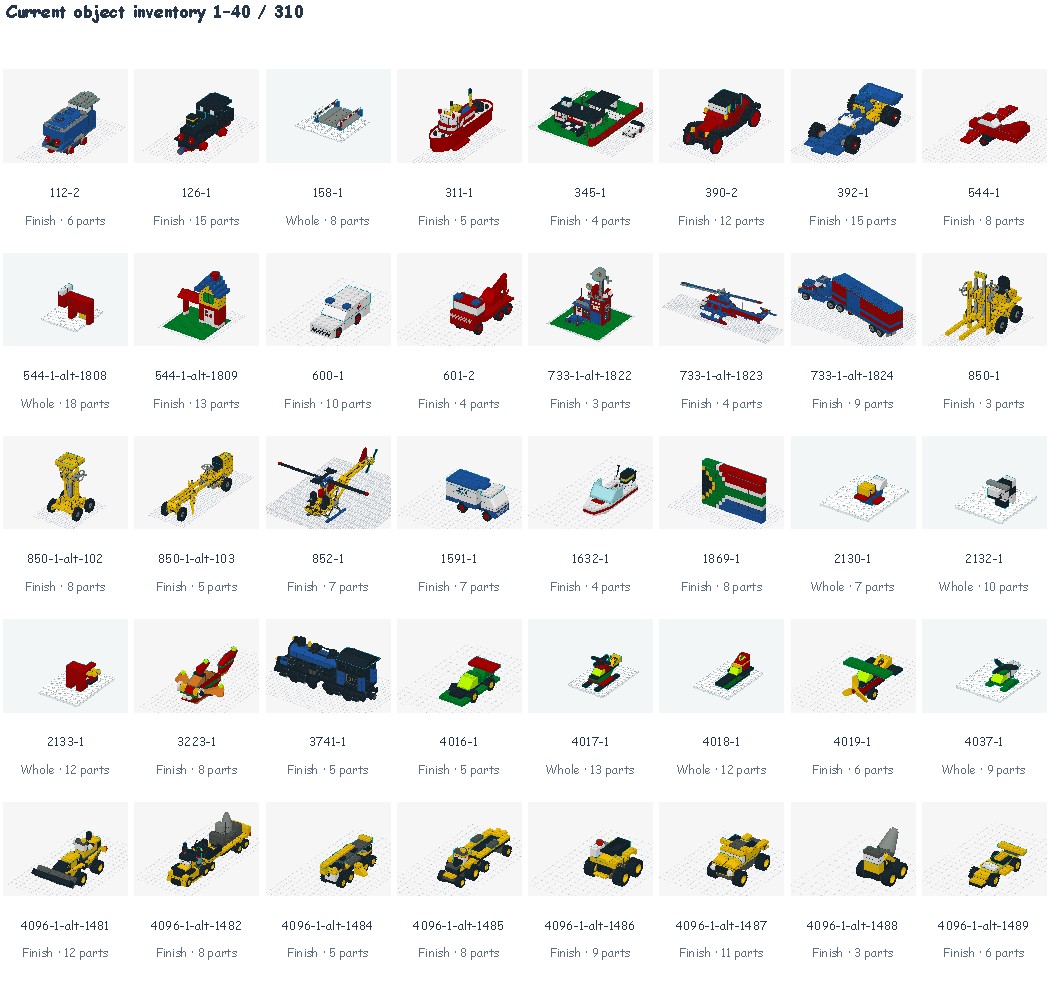
\includegraphics[width=\textwidth]{figures-release/gallery-1.pdf}\caption{Runnable object inventory, panel 1 of 8. Whole and Finish denote task scope; part counts refer to the operable target.}\end{figure}\clearpage
\begin{figure}[p]\centering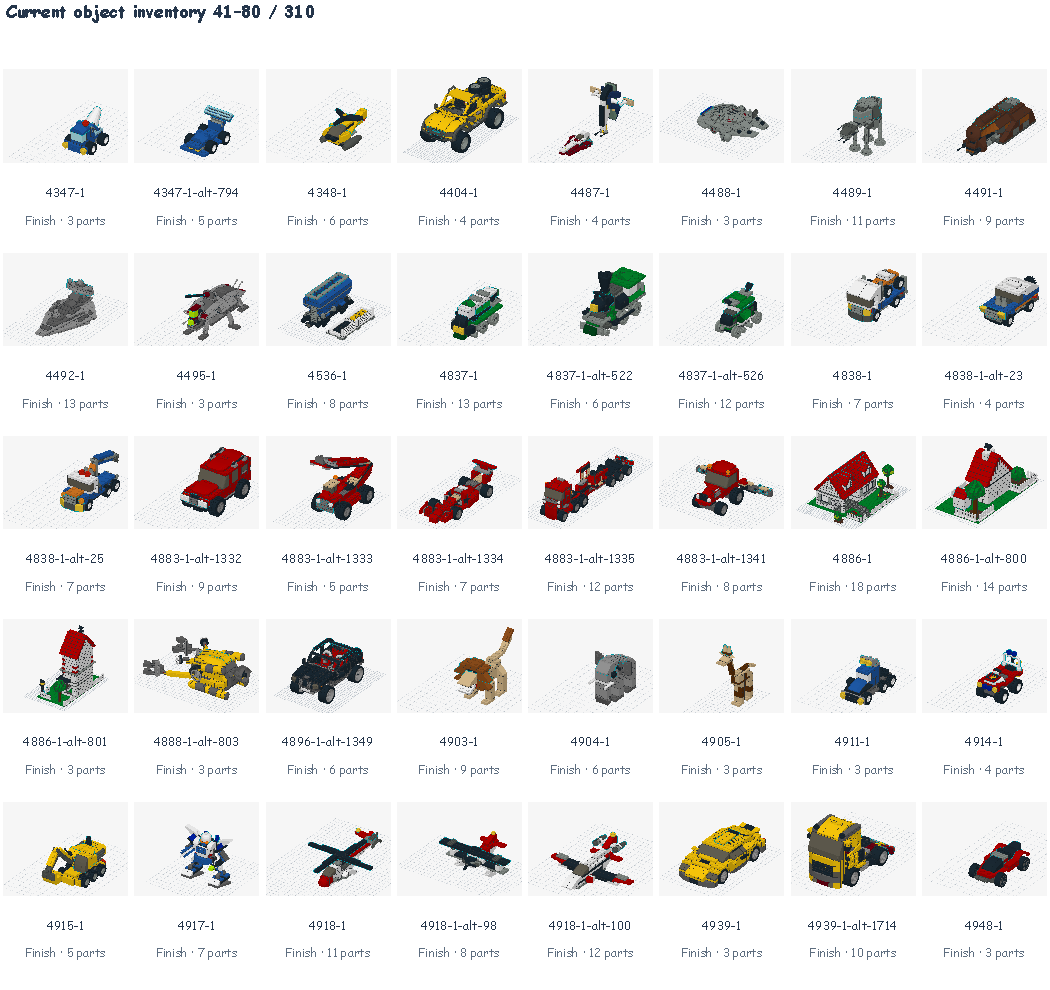
\includegraphics[width=\textwidth]{figures-release/gallery-2.pdf}\caption{Runnable object inventory, panel 2 of 8. Whole and Finish denote task scope; part counts refer to the operable target.}\end{figure}\clearpage
\begin{figure}[p]\centering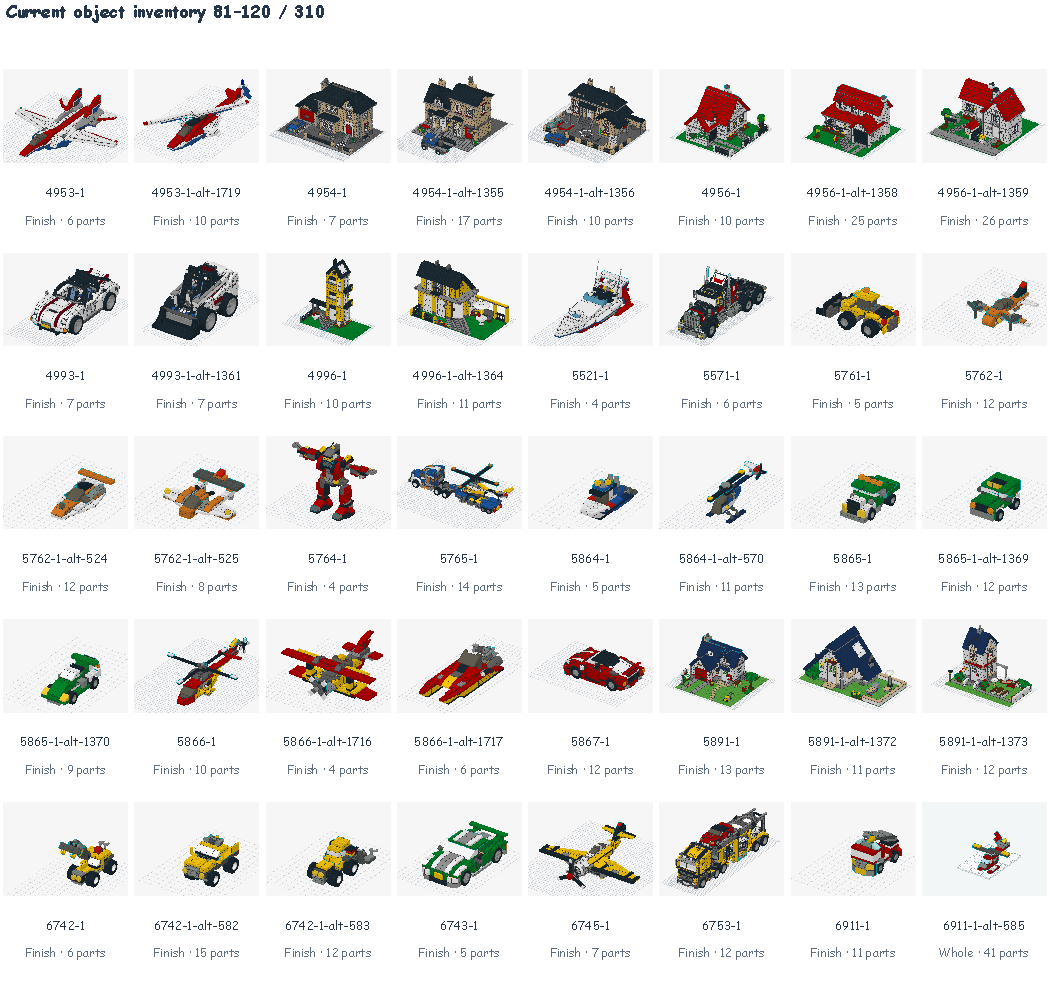
\includegraphics[width=\textwidth]{figures-release/gallery-3.pdf}\caption{Runnable object inventory, panel 3 of 8. Whole and Finish denote task scope; part counts refer to the operable target.}\end{figure}\clearpage
\begin{figure}[p]\centering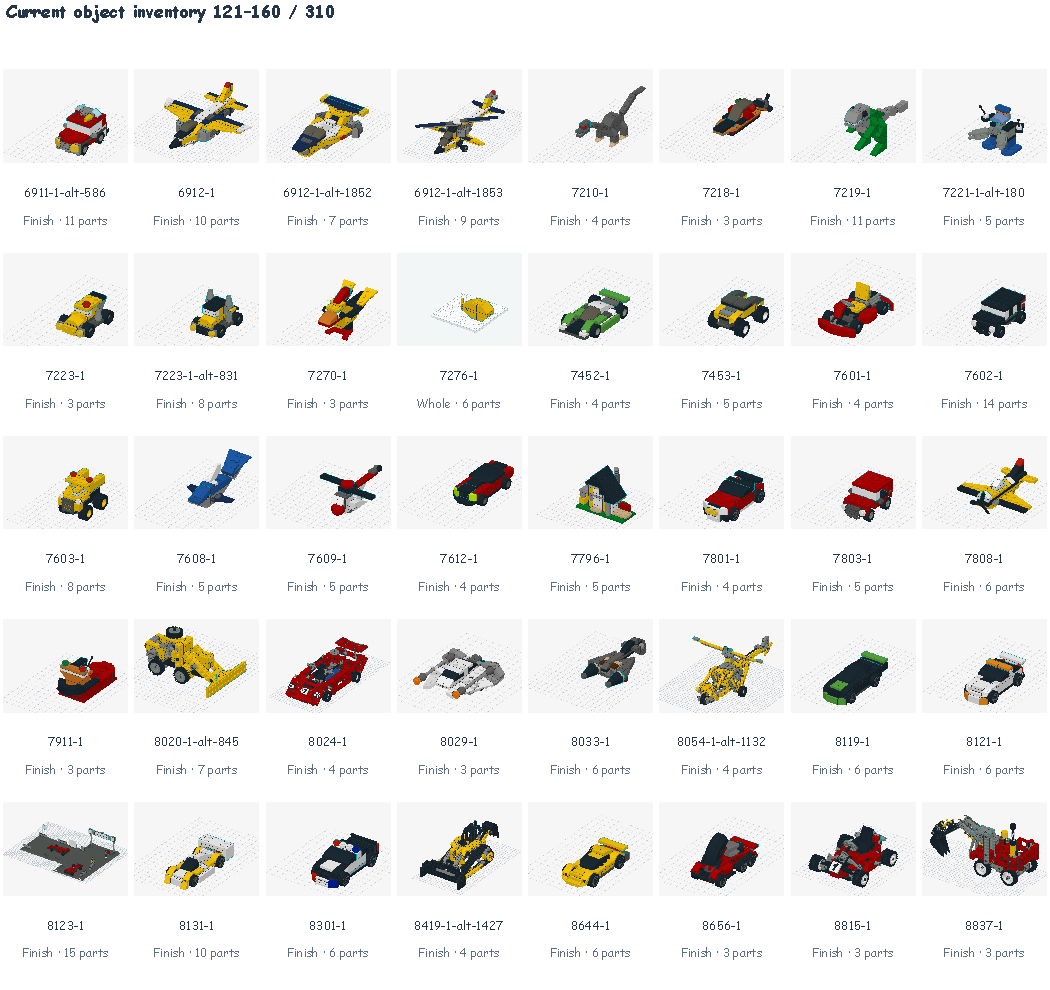
\includegraphics[width=\textwidth]{figures-release/gallery-4.pdf}\caption{Runnable object inventory, panel 4 of 8. Whole and Finish denote task scope; part counts refer to the operable target.}\end{figure}\clearpage
\begin{figure}[p]\centering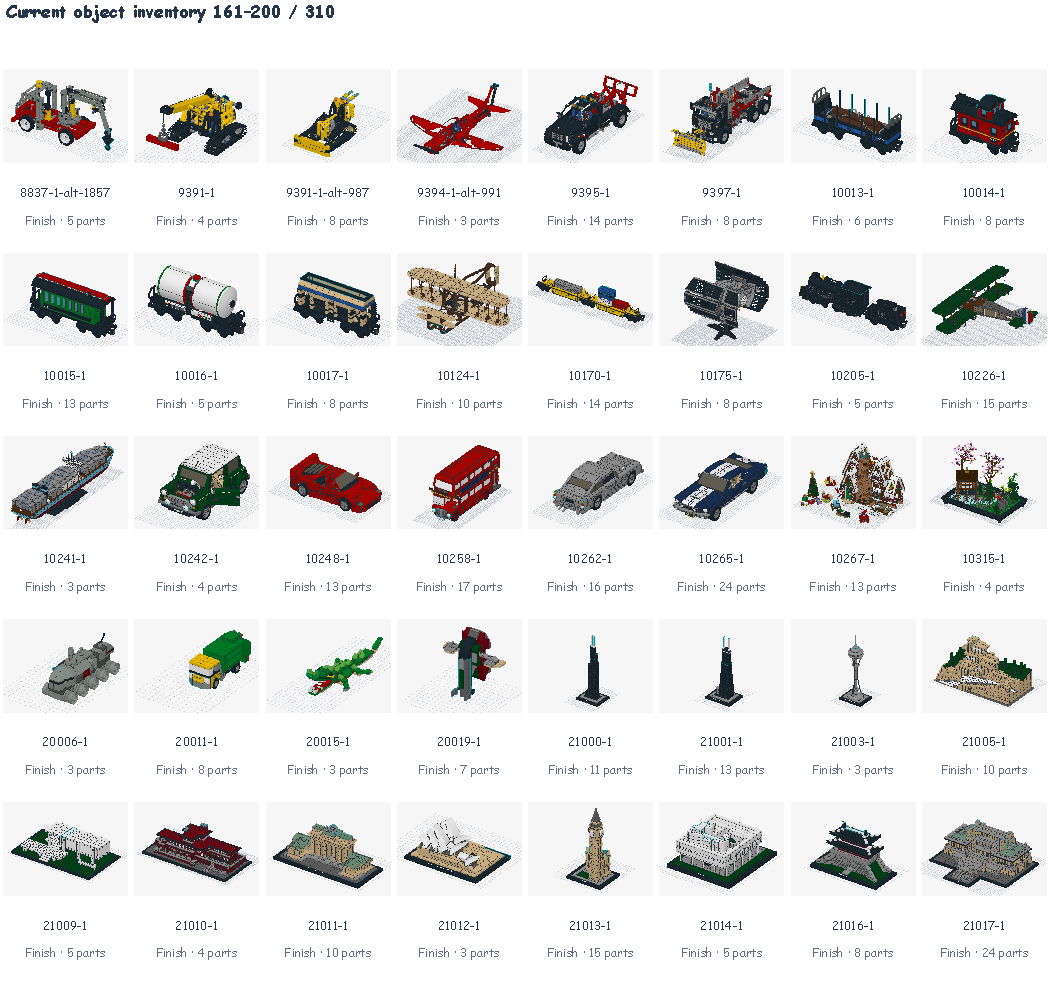
\includegraphics[width=\textwidth]{figures-release/gallery-5.pdf}\caption{Runnable object inventory, panel 5 of 8. Whole and Finish denote task scope; part counts refer to the operable target.}\end{figure}\clearpage
\begin{figure}[p]\centering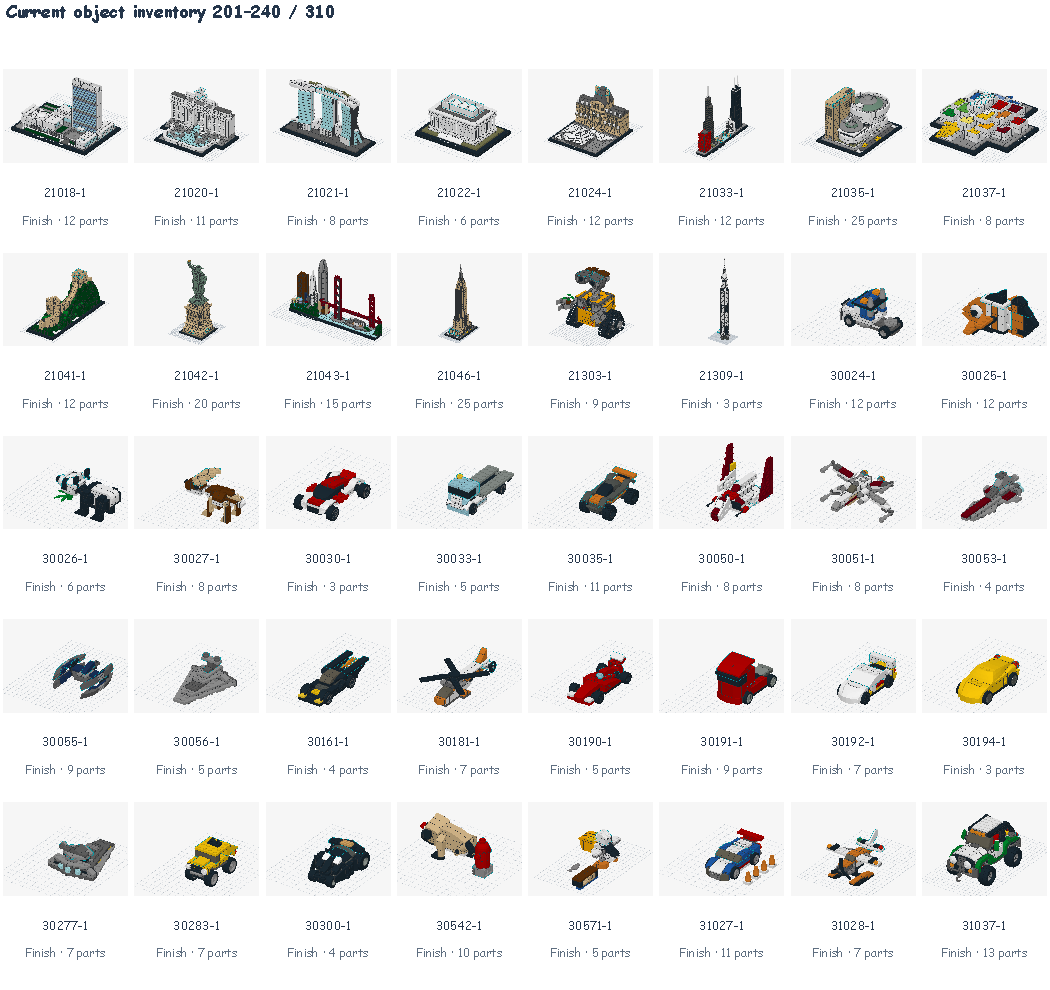
\includegraphics[width=\textwidth]{figures-release/gallery-6.pdf}\caption{Runnable object inventory, panel 6 of 8. Whole and Finish denote task scope; part counts refer to the operable target.}\end{figure}\clearpage
\begin{figure}[p]\centering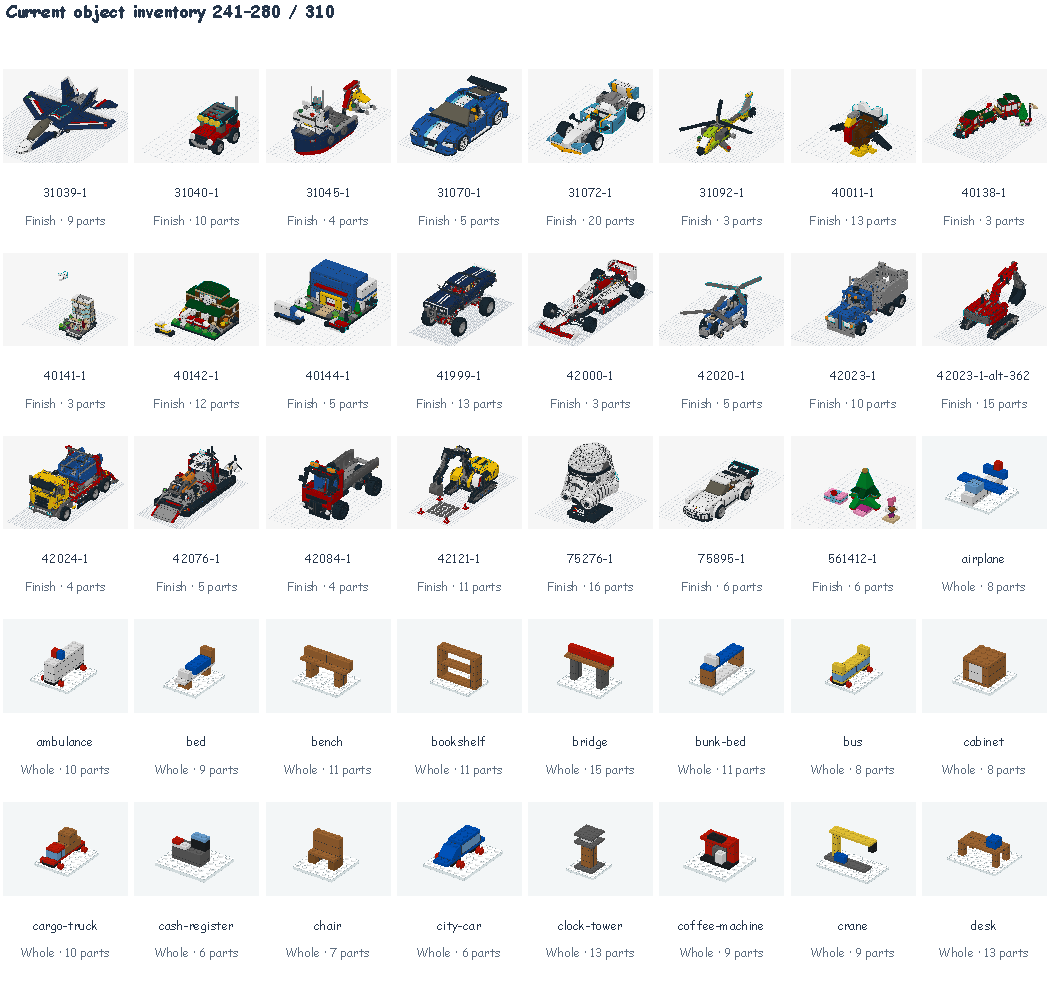
\includegraphics[width=\textwidth]{figures-release/gallery-7.pdf}\caption{Runnable object inventory, panel 7 of 8. Whole and Finish denote task scope; part counts refer to the operable target.}\end{figure}\clearpage
\begin{figure}[p]\centering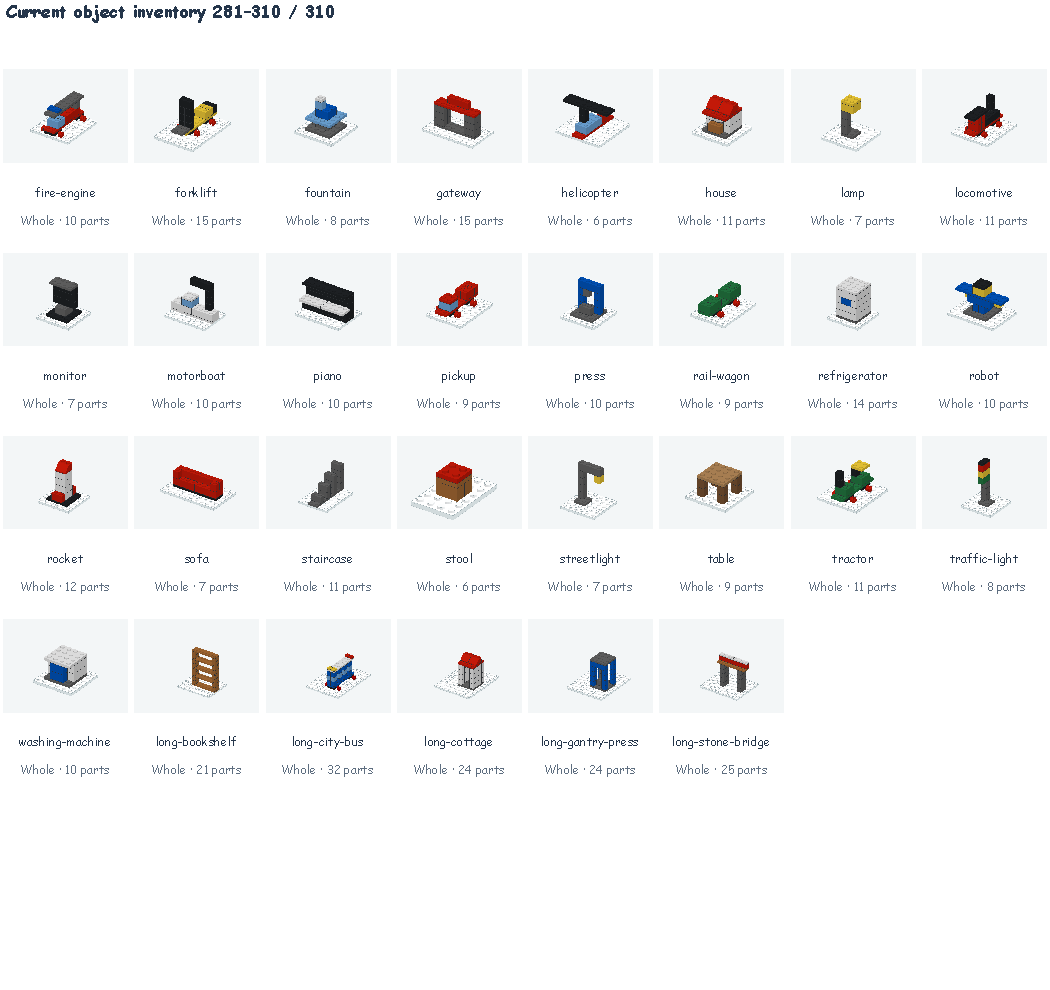
\includegraphics[width=\textwidth]{figures-release/gallery-8.pdf}\caption{Runnable object inventory, panel 8 of 8. Whole and Finish denote task scope; part counts refer to the operable target.}\end{figure}\clearpage

\clearpage
\small\begin{longtable}{@{}p{.40\textwidth}llrrr@{}}\caption{All 310 runnable object IDs. W: complete build; F: finishing task. S/M/L are length strata.}\\\toprule Object ID & Scope & Length & Parts & Static & Dynamic\\\midrule\endfirsthead\toprule Object ID & Scope & Length & Parts & Static & Dynamic\\\midrule\endhead
sc-112-2 & F & S & 6 & 6 & 6\\
sc-126-1 & F & M & 15 & 6 & 7\\
sc-158-1 & W & M & 8 & 6 & 7\\
sc-311-1 & F & S & 5 & 6 & 6\\
sc-345-1 & F & S & 4 & 3 & 3\\
sc-390-2 & F & M & 12 & 6 & 7\\
sc-392-1 & F & M & 15 & 6 & 7\\
sc-544-1 & F & M & 8 & 6 & 7\\
sc-544-1-alt-1808 & W & L & 18 & 6 & 7\\
sc-544-1-alt-1809 & F & M & 13 & 6 & 7\\
sc-600-1 & F & M & 10 & 6 & 7\\
sc-601-2 & F & S & 4 & 6 & 6\\
sc-733-1-alt-1822 & F & S & 3 & 2 & 2\\
sc-733-1-alt-1823 & F & S & 4 & 6 & 6\\
sc-733-1-alt-1824 & F & M & 9 & 6 & 7\\
sc-850-1 & F & S & 3 & 6 & 6\\
sc-850-1-alt-102 & F & M & 8 & 6 & 7\\
sc-850-1-alt-103 & F & S & 5 & 6 & 6\\
sc-852-1 & F & S & 7 & 6 & 6\\
sc-1591-1 & F & S & 7 & 6 & 6\\
sc-1632-1 & F & S & 4 & 6 & 6\\
sc-1869-1 & F & M & 8 & 6 & 7\\
sc-2130-1 & W & S & 7 & 6 & 6\\
sc-2132-1 & W & M & 10 & 6 & 7\\
sc-2133-1 & W & M & 12 & 6 & 7\\
sc-3223-1 & F & M & 8 & 6 & 7\\
sc-3741-1 & F & S & 5 & 6 & 6\\
sc-4016-1 & F & S & 5 & 6 & 6\\
sc-4017-1 & W & M & 13 & 6 & 7\\
sc-4018-1 & W & M & 12 & 6 & 7\\
sc-4019-1 & F & S & 6 & 6 & 6\\
sc-4037-1 & W & M & 9 & 6 & 7\\
sc-4096-1-alt-1481 & F & M & 12 & 6 & 7\\
sc-4096-1-alt-1482 & F & M & 8 & 5 & 6\\
sc-4096-1-alt-1484 & F & S & 5 & 6 & 6\\
sc-4096-1-alt-1485 & F & M & 8 & 6 & 7\\
sc-4096-1-alt-1486 & F & M & 9 & 6 & 7\\
sc-4096-1-alt-1487 & F & M & 11 & 6 & 7\\
sc-4096-1-alt-1488 & F & S & 3 & 2 & 2\\
sc-4096-1-alt-1489 & F & S & 6 & 6 & 6\\
sc-4347-1 & F & S & 3 & 6 & 6\\
sc-4347-1-alt-794 & F & S & 5 & 6 & 6\\
sc-4348-1 & F & S & 6 & 6 & 6\\
sc-4404-1 & F & S & 4 & 6 & 6\\
sc-4487-1 & F & S & 4 & 4 & 4\\
sc-4488-1 & F & S & 3 & 5 & 5\\
sc-4489-1 & F & M & 11 & 6 & 7\\
sc-4491-1 & F & M & 9 & 6 & 7\\
sc-4492-1 & F & M & 13 & 6 & 7\\
sc-4495-1 & F & S & 3 & 4 & 4\\
sc-4536-1 & F & M & 8 & 6 & 7\\
sc-4837-1 & F & M & 13 & 6 & 7\\
sc-4837-1-alt-522 & F & S & 6 & 5 & 5\\
sc-4837-1-alt-526 & F & M & 12 & 6 & 7\\
sc-4838-1 & F & S & 7 & 6 & 6\\
sc-4838-1-alt-23 & F & S & 4 & 6 & 6\\
sc-4838-1-alt-25 & F & S & 7 & 6 & 6\\
sc-4883-1-alt-1332 & F & M & 9 & 6 & 7\\
sc-4883-1-alt-1333 & F & S & 5 & 6 & 6\\
sc-4883-1-alt-1334 & F & S & 7 & 6 & 6\\
sc-4883-1-alt-1335 & F & M & 12 & 6 & 7\\
sc-4883-1-alt-1341 & F & M & 8 & 5 & 6\\
sc-4886-1 & F & L & 18 & 6 & 7\\
sc-4886-1-alt-800 & F & M & 14 & 6 & 7\\
sc-4886-1-alt-801 & F & S & 3 & 6 & 6\\
sc-4888-1-alt-803 & F & S & 3 & 6 & 6\\
sc-4896-1-alt-1349 & F & S & 6 & 6 & 6\\
sc-4903-1 & F & M & 9 & 6 & 7\\
sc-4904-1 & F & S & 6 & 6 & 6\\
sc-4905-1 & F & S & 3 & 5 & 5\\
sc-4911-1 & F & S & 3 & 4 & 4\\
sc-4914-1 & F & S & 4 & 6 & 6\\
sc-4915-1 & F & S & 5 & 6 & 6\\
sc-4917-1 & F & S & 7 & 6 & 6\\
sc-4918-1 & F & M & 11 & 6 & 7\\
sc-4918-1-alt-98 & F & M & 8 & 6 & 7\\
sc-4918-1-alt-100 & F & M & 12 & 6 & 7\\
sc-4939-1 & F & S & 3 & 5 & 5\\
sc-4939-1-alt-1714 & F & M & 10 & 6 & 7\\
sc-4948-1 & F & S & 3 & 4 & 4\\
sc-4953-1 & F & S & 6 & 6 & 6\\
sc-4953-1-alt-1719 & F & M & 10 & 6 & 7\\
sc-4954-1 & F & S & 7 & 6 & 6\\
sc-4954-1-alt-1355 & F & L & 17 & 6 & 7\\
sc-4954-1-alt-1356 & F & M & 10 & 6 & 7\\
sc-4956-1 & F & M & 10 & 6 & 7\\
sc-4956-1-alt-1358 & F & L & 25 & 6 & 7\\
sc-4956-1-alt-1359 & F & L & 26 & 6 & 7\\
sc-4993-1 & F & S & 7 & 6 & 6\\
sc-4993-1-alt-1361 & F & S & 7 & 6 & 6\\
sc-4996-1 & F & M & 10 & 6 & 7\\
sc-4996-1-alt-1364 & F & M & 11 & 6 & 7\\
sc-5521-1 & F & S & 4 & 5 & 5\\
sc-5571-1 & F & S & 6 & 6 & 6\\
sc-5761-1 & F & S & 5 & 6 & 6\\
sc-5762-1 & F & M & 12 & 6 & 7\\
sc-5762-1-alt-524 & F & M & 12 & 6 & 7\\
sc-5762-1-alt-525 & F & M & 8 & 6 & 7\\
sc-5764-1 & F & S & 4 & 6 & 6\\
sc-5765-1 & F & M & 14 & 6 & 7\\
sc-5864-1 & F & S & 5 & 6 & 6\\
sc-5864-1-alt-570 & F & M & 11 & 6 & 7\\
sc-5865-1 & F & M & 13 & 6 & 7\\
sc-5865-1-alt-1369 & F & M & 12 & 6 & 7\\
sc-5865-1-alt-1370 & F & M & 9 & 6 & 7\\
sc-5866-1 & F & M & 10 & 6 & 7\\
sc-5866-1-alt-1716 & F & S & 4 & 5 & 5\\
sc-5866-1-alt-1717 & F & S & 6 & 6 & 6\\
sc-5867-1 & F & M & 12 & 6 & 6\\
sc-5891-1 & F & M & 13 & 6 & 7\\
sc-5891-1-alt-1372 & F & M & 11 & 6 & 7\\
sc-5891-1-alt-1373 & F & M & 12 & 6 & 7\\
sc-6742-1 & F & S & 6 & 6 & 6\\
sc-6742-1-alt-582 & F & M & 15 & 6 & 7\\
sc-6742-1-alt-583 & F & M & 12 & 6 & 7\\
sc-6743-1 & F & S & 5 & 6 & 6\\
sc-6745-1 & F & S & 7 & 6 & 6\\
sc-6753-1 & F & M & 12 & 6 & 7\\
sc-6911-1 & F & M & 11 & 6 & 7\\
sc-6911-1-alt-585 & W & L & 41 & 6 & 7\\
sc-6911-1-alt-586 & F & M & 11 & 6 & 7\\
sc-6912-1 & F & M & 10 & 6 & 7\\
sc-6912-1-alt-1852 & F & S & 7 & 5 & 5\\
sc-6912-1-alt-1853 & F & M & 9 & 6 & 7\\
sc-7210-1 & F & S & 4 & 6 & 6\\
sc-7218-1 & F & S & 3 & 6 & 6\\
sc-7219-1 & F & M & 11 & 6 & 7\\
sc-7221-1-alt-180 & F & S & 5 & 6 & 6\\
sc-7223-1 & F & S & 3 & 6 & 6\\
sc-7223-1-alt-831 & F & M & 8 & 6 & 7\\
sc-7270-1 & F & S & 3 & 3 & 3\\
sc-7276-1 & W & S & 6 & 6 & 6\\
sc-7452-1 & F & S & 4 & 6 & 6\\
sc-7453-1 & F & S & 5 & 6 & 6\\
sc-7601-1 & F & S & 4 & 3 & 3\\
sc-7602-1 & F & M & 14 & 6 & 7\\
sc-7603-1 & F & M & 8 & 6 & 7\\
sc-7608-1 & F & S & 5 & 6 & 6\\
sc-7609-1 & F & S & 5 & 6 & 6\\
sc-7612-1 & F & S & 4 & 5 & 5\\
sc-7796-1 & F & S & 5 & 6 & 6\\
sc-7801-1 & F & S & 4 & 6 & 6\\
sc-7803-1 & F & S & 5 & 6 & 6\\
sc-7808-1 & F & S & 6 & 6 & 6\\
sc-7911-1 & F & S & 3 & 6 & 6\\
sc-8020-1-alt-845 & F & S & 7 & 6 & 6\\
sc-8024-1 & F & S & 4 & 4 & 4\\
sc-8029-1 & F & S & 3 & 6 & 6\\
sc-8033-1 & F & S & 6 & 4 & 4\\
sc-8054-1-alt-1132 & F & S & 4 & 6 & 6\\
sc-8119-1 & F & S & 6 & 6 & 6\\
sc-8121-1 & F & S & 6 & 6 & 6\\
sc-8123-1 & F & M & 15 & 6 & 7\\
sc-8131-1 & F & M & 10 & 6 & 7\\
sc-8301-1 & F & S & 6 & 6 & 6\\
sc-8419-1-alt-1427 & F & S & 4 & 2 & 2\\
sc-8644-1 & F & S & 6 & 6 & 6\\
sc-8656-1 & F & S & 3 & 5 & 5\\
sc-8815-1 & F & S & 3 & 3 & 3\\
sc-8837-1 & F & S & 3 & 6 & 6\\
sc-8837-1-alt-1857 & F & S & 5 & 6 & 6\\
sc-9391-1 & F & S & 4 & 3 & 3\\
sc-9391-1-alt-987 & F & M & 8 & 4 & 5\\
sc-9394-1-alt-991 & F & S & 3 & 5 & 5\\
sc-9395-1 & F & M & 14 & 6 & 7\\
sc-9397-1 & F & M & 8 & 4 & 4\\
sc-10013-1 & F & S & 6 & 5 & 5\\
sc-10014-1 & F & M & 8 & 6 & 7\\
sc-10015-1 & F & M & 13 & 5 & 6\\
sc-10016-1 & F & S & 5 & 6 & 6\\
sc-10017-1 & F & M & 8 & 5 & 6\\
sc-10124-1 & F & M & 10 & 6 & 7\\
sc-10170-1 & F & M & 14 & 6 & 7\\
sc-10175-1 & F & M & 8 & 3 & 4\\
sc-10205-1 & F & S & 5 & 6 & 6\\
sc-10226-1 & F & M & 15 & 6 & 7\\
sc-10241-1 & F & S & 3 & 2 & 2\\
sc-10242-1 & F & S & 4 & 3 & 3\\
sc-10248-1 & F & M & 13 & 5 & 6\\
sc-10258-1 & F & L & 17 & 6 & 7\\
sc-10262-1 & F & L & 16 & 6 & 6\\
sc-10265-1 & F & L & 24 & 6 & 7\\
sc-10267-1 & F & M & 13 & 6 & 6\\
sc-10315-1 & F & S & 4 & 2 & 2\\
sc-20006-1 & F & S & 3 & 5 & 5\\
sc-20011-1 & F & M & 8 & 6 & 7\\
sc-20015-1 & F & S & 3 & 6 & 6\\
sc-20019-1 & F & S & 7 & 6 & 6\\
sc-21000-1 & F & M & 11 & 6 & 7\\
sc-21001-1 & F & M & 13 & 5 & 6\\
sc-21003-1 & F & S & 3 & 2 & 2\\
sc-21005-1 & F & M & 10 & 6 & 7\\
sc-21009-1 & F & S & 5 & 6 & 6\\
sc-21010-1 & F & S & 4 & 5 & 5\\
sc-21011-1 & F & M & 10 & 6 & 7\\
sc-21012-1 & F & S & 3 & 4 & 4\\
sc-21013-1 & F & M & 15 & 6 & 7\\
sc-21014-1 & F & S & 5 & 6 & 6\\
sc-21016-1 & F & M & 8 & 6 & 7\\
sc-21017-1 & F & L & 24 & 6 & 7\\
sc-21018-1 & F & M & 12 & 6 & 7\\
sc-21020-1 & F & M & 11 & 6 & 7\\
sc-21021-1 & F & M & 8 & 6 & 7\\
sc-21022-1 & F & S & 6 & 6 & 6\\
sc-21024-1 & F & M & 12 & 6 & 7\\
sc-21033-1 & F & M & 12 & 6 & 7\\
sc-21035-1 & F & L & 25 & 6 & 7\\
sc-21037-1 & F & M & 8 & 4 & 5\\
sc-21041-1 & F & M & 12 & 6 & 7\\
sc-21042-1 & F & L & 20 & 6 & 7\\
sc-21043-1 & F & M & 15 & 6 & 7\\
sc-21046-1 & F & L & 25 & 6 & 7\\
sc-21303-1 & F & M & 9 & 6 & 7\\
sc-21309-1 & F & S & 3 & 5 & 5\\
sc-30024-1 & F & M & 12 & 6 & 7\\
sc-30025-1 & F & M & 12 & 6 & 7\\
sc-30026-1 & F & S & 6 & 6 & 6\\
sc-30027-1 & F & M & 8 & 6 & 7\\
sc-30030-1 & F & S & 3 & 5 & 5\\
sc-30033-1 & F & S & 5 & 6 & 6\\
sc-30035-1 & F & M & 11 & 6 & 7\\
sc-30050-1 & F & M & 8 & 5 & 6\\
sc-30051-1 & F & M & 8 & 6 & 7\\
sc-30053-1 & F & S & 4 & 6 & 6\\
sc-30055-1 & F & M & 9 & 6 & 7\\
sc-30056-1 & F & S & 5 & 6 & 6\\
sc-30161-1 & F & S & 4 & 6 & 6\\
sc-30181-1 & F & S & 7 & 6 & 6\\
sc-30190-1 & F & S & 5 & 6 & 6\\
sc-30191-1 & F & M & 9 & 6 & 6\\
sc-30192-1 & F & S & 7 & 6 & 6\\
sc-30194-1 & F & S & 3 & 3 & 3\\
sc-30277-1 & F & S & 7 & 6 & 6\\
sc-30283-1 & F & S & 7 & 6 & 6\\
sc-30300-1 & F & S & 4 & 6 & 6\\
sc-30542-1 & F & M & 10 & 5 & 6\\
sc-30571-1 & F & S & 5 & 6 & 6\\
sc-31027-1 & F & M & 11 & 6 & 7\\
sc-31028-1 & F & S & 7 & 6 & 6\\
sc-31037-1 & F & M & 13 & 6 & 7\\
sc-31039-1 & F & M & 9 & 6 & 7\\
sc-31040-1 & F & M & 10 & 6 & 7\\
sc-31045-1 & F & S & 4 & 6 & 6\\
sc-31070-1 & F & S & 5 & 6 & 6\\
sc-31072-1 & F & L & 20 & 6 & 7\\
sc-31092-1 & F & S & 3 & 2 & 2\\
sc-40011-1 & F & M & 13 & 6 & 7\\
sc-40138-1 & F & S & 3 & 4 & 4\\
sc-40141-1 & F & S & 3 & 5 & 5\\
sc-40142-1 & F & M & 12 & 6 & 7\\
sc-40144-1 & F & S & 5 & 5 & 5\\
sc-41999-1 & F & M & 13 & 6 & 7\\
sc-42000-1 & F & S & 3 & 6 & 6\\
sc-42020-1 & F & S & 5 & 6 & 6\\
sc-42023-1 & F & M & 10 & 6 & 7\\
sc-42023-1-alt-362 & F & M & 15 & 6 & 7\\
sc-42024-1 & F & S & 4 & 5 & 5\\
sc-42076-1 & F & S & 5 & 6 & 6\\
sc-42084-1 & F & S & 4 & 6 & 6\\
sc-42121-1 & F & M & 11 & 6 & 7\\
sc-75276-1 & F & L & 16 & 6 & 7\\
sc-75895-1 & F & S & 6 & 6 & 6\\
sc-561412-1 & F & S & 6 & 6 & 6\\
obj-airplane & W & M & 8 & 0 & 38\\
obj-ambulance & W & M & 10 & 0 & 25\\
obj-bed & W & M & 9 & 0 & 38\\
obj-bench & W & M & 11 & 0 & 32\\
obj-bookshelf & W & M & 11 & 0 & 47\\
obj-bridge & W & M & 15 & 0 & 28\\
obj-bunk-bed & W & M & 11 & 0 & 23\\
obj-bus & W & M & 8 & 0 & 29\\
obj-cabinet & W & M & 8 & 0 & 45\\
obj-cargo-truck & W & M & 10 & 0 & 41\\
obj-cash-register & W & S & 6 & 0 & 19\\
obj-chair & W & S & 7 & 0 & 20\\
obj-city-car & W & S & 6 & 0 & 21\\
obj-clock-tower & W & M & 13 & 0 & 46\\
obj-coffee-machine & W & M & 9 & 0 & 28\\
obj-crane & W & M & 9 & 0 & 23\\
obj-desk & W & M & 13 & 0 & 40\\
obj-fire-engine & W & M & 10 & 0 & 35\\
obj-forklift & W & M & 15 & 0 & 39\\
obj-fountain & W & M & 8 & 0 & 32\\
obj-gateway & W & M & 15 & 0 & 36\\
obj-helicopter & W & S & 6 & 0 & 17\\
obj-house & W & M & 11 & 0 & 41\\
obj-lamp & W & S & 7 & 0 & 14\\
obj-locomotive & W & M & 11 & 0 & 36\\
obj-monitor & W & S & 7 & 0 & 20\\
obj-motorboat & W & M & 10 & 0 & 23\\
obj-piano & W & M & 10 & 0 & 40\\
obj-pickup & W & M & 9 & 0 & 37\\
obj-press & W & M & 10 & 0 & 45\\
obj-rail-wagon & W & M & 9 & 0 & 37\\
obj-refrigerator & W & M & 14 & 0 & 45\\
obj-robot & W & M & 10 & 0 & 38\\
obj-rocket & W & M & 12 & 0 & 57\\
obj-sofa & W & S & 7 & 0 & 22\\
obj-staircase & W & M & 11 & 0 & 40\\
obj-stool & W & S & 6 & 0 & 17\\
obj-streetlight & W & S & 7 & 0 & 13\\
obj-table & W & M & 9 & 0 & 31\\
obj-tractor & W & M & 11 & 0 & 35\\
obj-traffic-light & W & M & 8 & 0 & 23\\
obj-washing-machine & W & M & 10 & 0 & 50\\
v7-long-bookshelf & W & L & 21 & 24 & 23\\
v7-long-city-bus & W & L & 32 & 24 & 23\\
v7-long-cottage & W & L & 24 & 22 & 23\\
v7-long-gantry-press & W & L & 24 & 26 & 25\\
v7-long-stone-bridge & W & L & 25 & 26 & 23\\
\bottomrule\end{longtable}

\end{document}
